\chapter{Prefix sum}
\label{sec:prefix_sum}

The all-prefix-sums operation (also referred to as prefix sum or simply scan) is a simple calculation which is most often found as part of larger and more complex routines. It serves as fundamental building block for implementing well-known algorithms such as radix sort (covered in section \ref{sec:sorting_radix}), stream compacting, minimum spanning tree and many more (cf. Blelloch's papers on prefix sum \cite{scan_blelloch_examples} \cite{scan_blelloch} and the GPU Gems 3 book section 39.1 \cite{gpu_gems_3_chapter_39}).

The all-prefix-sums operation uses a binary, associative operator $\oplus$ with identity element $I$ to transform an input array of $n$ elements
\begin{equation*}
[a_0, a_1, \dots, a_{n-1}]
\end{equation*}
into an output array of $n$ elements where

\begin{enumerate}[label=\alph*)]
	\item 
	each output element is the sum of all elements preceding the corresponding input element. This is known as an exclusive scan. \cite{gpu_gems_3_chapter_39}
	\begin{equation*}
	[I, a_0, (a_0 \oplus a_1), \dots, (a_0 \oplus a_1 \oplus \dots \oplus a_{n-2})]
	\end{equation*}
	
	\item
	each  output element is the sum of all elements preceding the corresponding input element and the input element itself. This is known as an inclusive scan. \cite{gpu_gems_3_chapter_39}
	\begin{equation*}
	[a_0, (a_0 \oplus a_1), \dots, (a_0 \oplus a_1 \oplus \dots \oplus a_{n-1})]
	\end{equation*}
\end{enumerate}

Contrary to the matrix multiplication of chapter \ref{sec:matrix_mul}, the all-prefix-sums operation does not offer similarly trivial parallelism. Scanning an array is naturally sequential with a complexity of $\mathcal{O}(n)$. Although each output element could be calculated independently to gain parallelism, a lot of redundant work would be necessary raising the overall complexity to $\mathcal{O}(n^2)$ with the last element still taking $\mathcal{O}(n)$ time to calculate.
This chapter will focus on efficient and parallel implementations of exclusive scan (except otherwise noted) using addition as operator on an input array of signed 32 bit integers. This chapter is orientated towards the Parallel Prefix Sum article from GPU Gems 3 \cite{gpu_gems_3_chapter_39}.

\begin{figure}[!p]
\centering
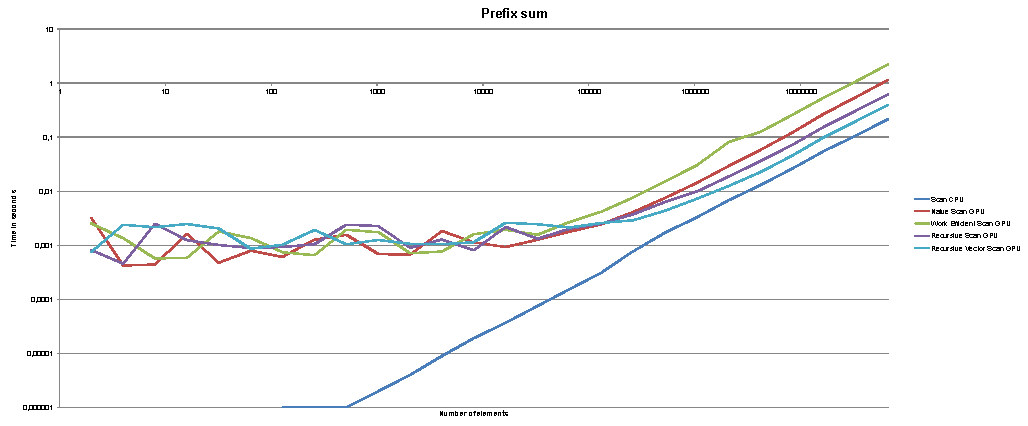
\includegraphics[width=0.9\textheight, angle=90]{scan_chart}
\caption{Benchmark of several prefix sum implementations, where
%The chart is based on the benchmark data in appendix section \ref{sec:scan_chart_data}.
both axes are of logarithmic scale.}
\label{fig:scan_chart}
\end{figure}

\section{CPU Implementation}
\label{sec:scan_cpu}

Implementing a sequential, single threaded scan for the CPU is simple. The first output element is initialized to zero. We than loop over the remaining output elements and set each one to the value of its predecessor plus the corresponding input element. Listing \ref{lst:scan_cpu} presents an example of a scan implementation.

\lstset{basicstyle=\ttfamily{}\scriptsize{}}
\lstinputlisting[language=CPP, caption=A simple C++ implementation of an exclusive scan for the CPU., label=lst:scan_cpu, firstline=34, lastline=38]{code/scan/main.cpp}
\lstset{basicstyle=\ttfamily{}}

This code performs exactly $n - 1$ additions which is the minimum number of additions required to produce an exclusive scan of an array with $n$ elements. Concerning the following parallel scan implementations later in this chapter, we would like them to be work-efficient. This means that the parallel implementation should have the same work complexity of $\mathcal{O}(n)$ as the sequential one.

\begin{quote}
A parallel computation is work-efficient if it does asymptotically no more work (add operations, in this case) than the sequential version \cite{gpu_gems_3_chapter_39}.
\end{quote}

The benchmark of this algorithm in figure \ref{fig:scan_chart} confirms the linearity of scan. Furthermore, we can also see that scanning is a quite fast operation (when, e.g., being compared to the matrix multiplication of chapter \ref{sec:matrix_mul}). The CPU implementation manages to scan $2^{26}$ elements (256 MiB of data) in 225 ms.


\section{Naive GPU implementation}
\label{sec:scan_naive}

The first GPU implementation is base on the article Data Parallel Algorithms \cite{scan_naive}. The discussed approach is to compute an inclusive (!) scan is shown in figure \ref{fig:scan_naive}. The algorithm uses several passes to compute the final output array in place. In each pass the value of a predecessor is added to an element. The offset from each element to its predecessor is determined by the pass index and is $2^{d - 1}$ where d is the number of the pass starting with 1.

\begin{figure}[h]
\centering
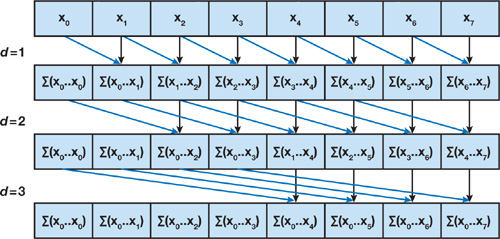
\includegraphics[width=0.6\textwidth]{scan_naive}
\caption{A naive approach for a parallel scan. \cite{gpu_gems_3_chapter_39}}
\label{fig:scan_naive}
\end{figure}

By now the algorithm assumes that in each pass all input elements are read before any output elements are written. This can only be achieved if this algorithm is run on a device with as many cores as input elements to ensure correct read and write ordering. This is usually not the case for larger arrays (current GPUs have around a few thousands cores. cf. NVIDIA Kepler GK110 in section \ref{sec:gpu}). A solution to this problem is double buffering. Instead of computing the partial sums in place inside the input array, a second, equally sized buffer is created. In each pass input data is read from one of the buffers and written to the other. Before the next pass the buffers are swapped.
Listing \ref{lst:scan_naive_host} shows an example host code implementing this approach.

\lstset{basicstyle=\ttfamily{}\scriptsize{}}
\lstinputlisting[language=CPP, caption=Host code for the naive scan algorithm., label=lst:scan_naive_host, firstline=40, lastline=64]{code/scan/main.cpp}
\lstset{basicstyle=\ttfamily{}}

At first, two buffers with the size of the input are created. Both of them have to be read- and writable as they are read from and written to alternatingly when executing the passes. The source buffer is filled with the input data. Although this algorithm is independent from the chosen work group size, we have to round the number of enqueued work items (one for each input element) up to be a multiple of the work group size, which will be the size of the enqueued ND range. After this short setup the passes are executed. Each pass corresponds to a power of two (loop variable \lstinline!offset!, cf. figure \ref{fig:scan_naive}) which corresponds to the offset of an element to the predecessor that should be added to it. This offset is raised to the next power of two each pass until it is larger than the problem size. The kernel is executed once for each pass, given the source and destination buffer, the offset and the original problem size as arguments. At the end of a pass the source and destination buffers are swapped (only the handles, not the actual contents). After the last pass has been executed, the result is read from the source buffer (the last pass wrote to the destination buffer which was swapped with the source buffer at the end of the loop).
Listing \ref{lst:scan_naive_kernel} shows the kernel code corresponding to the host code from listing \ref{lst:scan_naive_host}.

\lstset{basicstyle=\ttfamily{}\scriptsize{}}
\lstinputlisting[language=CL, caption=OpenCL Kernel code for the naive scan algorithm., label=lst:scan_naive_kernel]{../src/scan/gpu/thesis/NaiveScan.cl}
\lstset{basicstyle=\ttfamily{}}

The kernel starts by querying the id of the current element. If this id is larger than the actual problem size, the kernel returns. This case can happen when the problem size has been rounded up to be a multiple of the chosen work group size. If the id addresses a valid input element, we determine if this element has a predecessor at the current pass' offset. If this is the case, the input element is read from the source buffer, added to its predecessor (also read from the source buffer) and written to the destination buffer. If the predecessor offset is to large, the input element remains the same, but has to be copied if it was just calculated in the last pass (to keep the buffers consistent).

When we have a look at the benchmark of this algorithm and compare the results with the CPU implementation, we can clearly see that this approach does not profit very well from the large computational power GPUs offer. With 1132 ms at $2^{26}$ elements the naive GPU version is five times slower than the CPU version. The low performance has basically two reasons. The first is the high number of kernel invocations necessary to compute the final result. For $2^{26}$ input elements to scan, 26 passes are necessary each consisting of $2^{26}$ work items mostly performing one addition. Hence, leading to a runtime/work complexity of $\mathcal{O}(n log n)$. Compared with the complexity of the original CPU implementation, which was $\mathcal{O}(n)$, this algorithm is not work-efficient. The second flaw of this implementation is the high rate of global memory access. Both buffers are accessed multiple times at the same locations throughout the passes. As the scan operation using a simple addition is more memory bound than computational, a lot of time is wasted on waiting for global memory transactions.
Fortunately, both problems can be tackled which will be subject to the following sections.


\section{Work efficient GPU implementation}
\label{sec:scan_work_efficient}

In 1990 Blelloch presented a more efficient version of the all-prefix-sums operation in his article Prefix Sums and Their Applications \cite{scan_blelloch}. He presented a tree-based approach consisting of three phases.

\begin{figure}[h]
\centering
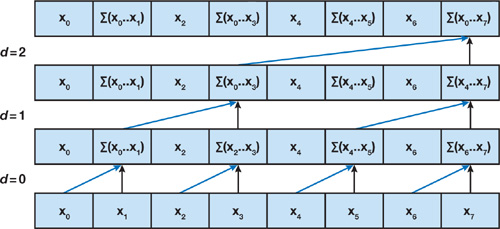
\includegraphics[width=0.6\textwidth]{scan_work_efficient_up_sweep}
\caption{The up-sweep phase of a work efficient parallel scan \cite{gpu_gems_3_chapter_39}}
\label{fig:scan_work_efficient_up_sweep}
\end{figure}

The first phase is called the reduce or up-sweep phase and is illustrated in figure \ref{fig:scan_work_efficient_up_sweep}. It takes an input array whose length must be a power of two. All elements of the input array are leaves of the tree. The algorithm than takes adjacent pairs of elements and adds them together forming a node holding the sum of it's two child nodes. This step forms a pass of the up-sweep phase and is repeated for the created parent nodes until the root of the tree which than holds the sum of all values. As the values of the right child nodes are not needed anymore after their parent nodes have been calculated, the tree can be built in-place.

\begin{figure}[h]
\centering
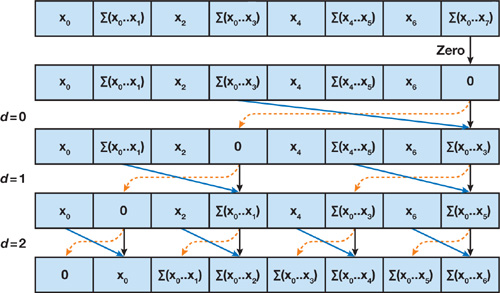
\includegraphics[width=0.6\linewidth]{scan_work_efficient_down_sweep}
\caption{The down-sweep phase of a work efficient parallel scan \cite{gpu_gems_3_chapter_39}}
\label{fig:scan_work_efficient_down_sweep}
\end{figure}

The second phase sets the value of the root node to zero to prepare for the third phase, the down-sweep phase, which is illustrated in figure \ref{fig:scan_work_efficient_down_sweep}. The down-sweep phase again consists of several passes starting at the root node and repeating along all levels of the tree until the leaves. In each pass the values of the left child nodes are read and temporarily stored. The left child nodes are than replaced by the value of their parent nodes. The previous, temporarily stored values of the left child nodes are then added to the parent nodes' values and written to the right child node. As the parent nodes are not needed anymore after the sum for the right child has been calculated, the tree can again be traversed downwards in-place.
Overall, for an input array of $n$ elements, this algorithm performs $n - 1$ adds during the up-sweep phase and the same amount of adds during the down-sweep phase\footnote{A perfect binary tree with $n$ leaves has a total of $2n - 1$ nodes. As only the non-leaf nodes perform additions, the number of leaf nodes can be subtracted resulting in $2n - 1 - n = n - 1$ nodes which perform an addition.}. Although almost twice as much work is performed when compared with the sequential CPU implementation, this algorithm can still be considered work-efficient according to the definition given in section \ref{sec:scan_cpu}.
Listing \ref{lst:scan_work_efficient_host} shows the host code implementing the work-efficient tree based approach after Blelloch \cite{scan_blelloch}.

\lstset{basicstyle=\ttfamily{}\scriptsize{}}
\lstinputlisting[language=CPP, caption=Host code for the work-efficient scan algorithm., label=lst:scan_work_efficient_host, firstline=66, lastline=103]{code/scan/main.cpp}
\lstset{basicstyle=\ttfamily{}}

Contrary to the previous algorithms, this implementation will use two kernels, one for the up-sweep and one for the down-sweep phase. 
To start with, the number of input elements has to be rounded up to be a power of two. This size is then used to create a buffer which is filled with the input array.
After these initialization steps we can begin with the up-sweep phase. The loop variable for the passes is the offset of the buffer index between two adjacent nodes on the same tree level. This value starts with one for the first pass and is raised to the next power of two for each subsequent pass until the size of the input buffer has been reached. For each pass the up-sweep kernel is enqueued with the buffer and the current pass' offset as arguments. The number of work items required for a pass is equal to the number of parent nodes calculated on the current pass' level. This value is a half of the buffer size for the first pass and halves itself after each pass. Although this algorithm is still independent of the chosen work group size, we have to make sure that it is not larger than the global number of work items. \\
After the up-sweep phase has been completed, the last element corresponding to the tree's root node will be set to zero. This is easily accomplished by enqueuing a write operation writing the value zero to the last buffer element. \\
Finally the down-sweep phase can finish the scan computation. Similar to the up-sweep phase several passes are executed given the offset between two adjacent tree nodes on the same level and the buffer as argument. In contrast to the up-sweep phase, the tree is now traversed top-down meaning the offset starts with a half of the buffer size and is set to the next lower power of two in each pass until one has been reached. Analogous, the number of nodes to process (the global work size) starts with one and doubles every pass.
When the down-sweep phase has completed, the buffer holds the final scan result which can than be read back to host memory.
Listing \ref{lst:scan_work_efficient_kernel} shows the corresponding OpenCL kernel code for the work-efficient scan implementation.

\lstset{basicstyle=\ttfamily{}\scriptsize{}}
\lstinputlisting[language=CL, caption=OpenCL Kernel code for the work efficient scan algorithm., label=lst:scan_work_efficient_kernel]{../src/scan/gpu/thesis/WorkEfficientScan.cl}
\lstset{basicstyle=\ttfamily{}}

The \lstinline!UpSweep! kernel starts by computing the value of \lstinline!stride! which is the distance of two parent nodes in the current pass. This value is used to calculate the buffer index (\lstinline!id!) of the current parent node (equal to the right child node) from the work items global id. The input value at \lstinline!id! is read (right child) together with the corresponding neighbor node at the given offset (left child). The computed sum is then written over the right child's location. \\
The \lstinline!DownSweep! kernel initializes the same way as it's preceding one by determining the current pass' stride and the parent node's index. Then, the value of the parent node is read and temporarily stored. The value of the left child node (given by \lstinline!offset!) is added the parent node (which becomes the right child node). Finally the previous, temporarily stored value of the parent node is passed down to the left child node.

When having a look at the benchmark results for this algorithm in figure \ref{fig:scan_chart} we can see that our efforts have payed off. The initial 1132 ms of the naive GPU implementation have shrunk to 604 ms on an array of $2^{26}$ elements. Furthermore, this implementation is now work-efficient and therefore avoiding unnecessary additions. Additionally, as all intermediate results are stored in-place, the algorithm does not waste memory by double buffering, such as the naive approach. However, the algorithm requires the input to be a power of two, which becomes more disadvantages with larger input sizes. %This can be clearly seen in the performance data table of the work-efficient scan in appendix section \ref{sec:scan_chart_data}, where the time required for the calculation is equal for all problem sizes that are round up to the same power of two. This also explains the stepped shape of the runtime curve.
This can be clearly seen at the stepped shape of the runtime curve which rises at every new power of two as the time required for the calculation is equal for all problem sizes that are round up to the same power of two.

\section{Recursively scanning blocks in local memory}
\label{sec:scan_recursive}

The previous work-efficient implementation in section \ref{sec:scan_work_efficient} does already perform quite well for an initially sequential problem. However, the input buffer size restriction is undesirable. Furthermore, no local memory is used which might be useful for computing and storing intermediate results.

\begin{figure}[h]
\centering
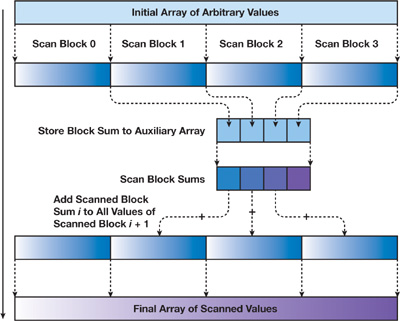
\includegraphics[width=0.5\linewidth]{scan_recursive}
\caption{Scanning larger arrays of values recursively \cite{gpu_gems_3_chapter_39}.}
\label{fig:scan_recursive}
\end{figure}

GPU Gems 3 Chapter 39 \cite{gpu_gems_3_chapter_39} shows a different approach for computing all prefix sums of an input array. The method is shown in figure \ref{fig:scan_recursive}. The input data is rounded up to be a multiple of a block size (which is two times the chosen work group size in their implementation). Each work group then loads a block from global memory to local memory. Each block is then scanned using Blelloch's work-efficient scan algorithm \cite{scan_blelloch}, but in local memory inside a work group. After the up-sweep phase is finished, the root element of each tree in a block is copied into a smaller, temporary buffer. This buffer is then recursively scanned again. The scan result of the temporary buffer can then be used to offset the scanned blocks of the original buffer to build the final scan.
Although this algorithm is not tied to a specific work group size it performs better the larger the work group size is chosen, as the work group sizes determines the factor by which the input data is reduced in each recursion.
Listing \ref{lst:scan_recursive_host} shows the host code of this recursive scan algorithm.

\lstset{basicstyle=\ttfamily{}\scriptsize{}}
\lstinputlisting[language=CPP, caption=Host code for the recursive scan algorithm., label=lst:scan_recursive_host, firstline=105, lastline=140]{code/scan/main.cpp}
\lstset{basicstyle=\ttfamily{}}

This implementation again uses two kernels, one for scanning the blocks in local memory and one for applying the offsets from the scanned temporary buffer to the original one. The host code consists of two parts, the setup code and the actual recursion. The setup is performed in \lstinline!recursiveGPU! which starts by rounding the input data size up to be a multiple of twice the size of a work group, because each work item processes two values. Then a buffer is created and the input data written to it. This buffer is then passed to the recursive scan procedure \lstinline!recursiveGPU_r!. The recursion starts by computing the size of the temporary buffer \lstinline!sums! that will hold the values of the root nodes (the sums over each block). As each thread processes two input elements and each work group computes one sum over a block, this temporary buffer's size is the problem size divided by two times the work group size. The result is then rounded up to be a multiple of this value, so it can be recursively scanned again with this algorithm. After the size has been determined, the \lstinline!sums! buffer can be created. No initialization or memory transfer is required as the buffer is entirely accessed by the kernels. Afterwards, the block scan kernel can be set up. It takes the original input buffer as well as the buffer for the sums as arguments. Furthermore local memory is allocated to cache the block calculated by each work group. As each work item reads two input elements, the global work size is half the number of input elements. After the kernel has been enqueued, we have to check whether the input data for this recursion consisted of more than one block. If this is the case we scan the temporary buffer (containing more than 1 value) by recursively calling \lstinline!recursiveGPU_r! on this buffer. After scanning the temporary \lstinline!sums! buffer has completed, the sums can be applied to the original buffer. Therefore another kernel is enqueued given both buffers as arguments. The global and local work size are equal to the previous kernel on the same recursion level.
Listing \ref{lst:scan_recursive_kernel} shows the kernel code for the recursive scan implementation.

\lstset{basicstyle=\ttfamily{}\scriptsize{}}
\lstinputlisting[language=CL, caption=OpenCL Kernel code for the recursive scan algorithm., label=lst:scan_recursive_kernel, firstline=1, lastline=55]{../src/scan/gpu/thesis/RecursiveScan.cl}
\lstset{basicstyle=\ttfamily{}}

The \lstinline!ScanBlocks! kernel starts with querying some values from OpenCL. Beside the global and local id, also the size \lstinline!n! of the block of the current work group is determined. Each thread than loads two values of the block into local memory. The following code then implements the tree based scan approach by Blelloch which has already been discussed in the previous section \ref{sec:scan_work_efficient}. The three phases (up-sweep, set-last-zero and down-sweep) are executed across all threads of the work group on the block in local memory. The only difference is, that the computed value of the root node after the up-sweep phase is moved to the \lstinline!sums! buffer at the index of the current work group. After the block has been scanned completely, it is copied back from local to global memory.

The \lstinline!AddSums! kernel is executed with the same global and local sizes as passed to the \lstinline!ScanBlocks! kernel on the same recursion level. The \lstinline!sums! buffer now contains a scan of the sums of all blocks scanned in this recursion. Therefore, the position where the \lstinline!ScanBlocks! kernel wrote the root node's value, now contains the sum of all elements (of all blocks) preceding the block of the current work group. This value is retrieved and added to all values of the current block finishing the scan.

Concerning the performance benchmark in figure \ref{fig:scan_chart}, this implementation scales better with the problem size although it is not faster than the global work-efficient scan of the previous section (606 vs. 604 ms on $2^{26} elements$). Furthermore, the recursive implementations' kernels are enqueued far less often than the one's of the work-efficient implementation. This can be explained by the reduction factor in each algorithm. The work efficient implementation reduces the number of work items by a factor of two each iteration while the recursive algorithm reduces by the work group size (which was 256 for the benchmarks) times two. In return, a lot more work is done inside the recursive algorithm's kernels. Also the number of additions required to compute the final result increased as extra adds a needed to apply the sums from the temporary buffer to the input buffer.
However, this implementation showed a different concept of how a problem can be broken down into smaller parallel pieces of work. The next implementation will follow up on this idea.

\section{Optimization using vector types}
\label{sec:scan_vector}

The final implementation shown in this chapter takes the idea of the recursive scan approach from the previous chapter one step further \cite[ch.39.2.5]{gpu_gems_3_chapter_39}. Instead of loading only two elements in each work item we will load two vectors of elements. These are then scanned inside each work item. The sums of the vectors (root node after the up-sweep phase) is then copied to local memory. The algorithm then continues just as the previous chapter's version by scanning the blocks in local memory. The results can then be used to offset the vectors of each work item just as the \lstinline!AddSums! kernel on a higher level. The remaining part of the implementation basically stays the same.
With this modification, each work group does not only load a block of two times the work group size of elements but a block of two times the work group size times the chosen vector width. As a result the input array is reduced faster by a factor of the chosen vector width in each recursion. The consumed local memory stays the same as only the sums of both vectors are placed into local memory. Only the consumed registers will increase.
Listing \ref{lst:scan_recursive_vector_host} shows the differences of the host code of the this vector type implementation compared with the previous one.

\lstset{basicstyle=\ttfamily{}\scriptsize{}}
\lstinputlisting[language=CPP, caption=Differences to the host code shown in listing \ref{lst:scan_recursive_kernel} for the recursive scan algorithm using vector types., label=lst:scan_recursive_vector_host, firstline=143, lastline=152]{code/scan/main.cpp}
\lstset{basicstyle=\ttfamily{}}

The first and most important step is to define the width of the vectors used. OpenCL supports vector types with the lengths of 2, 4, 8 or 16. The larger this \lstinline!VECTOR_WIDTH! is chosen, the larger is the reduction of the input buffer in each recursion. However, as a side effect the consumed registers per work item increase leading to a lower occupancy of the kernel. The ideal vector width may be hardware specific and is subject to corresponding benchmarks. This implementation will use a \lstinline!VECTOR_WIDTH! of 8.
The remaining changes to the host code are straight forward. As the blocks get bigger by a factor of \lstinline!VECTOR_WIDTH!, the size of the temporary \lstinline!sums! buffer decreases by and has to be rounded up to the same factor. Furthermore, the global work size shrinks. Finally, the check whether the input array consisted of more than one block has to be adapted to the new block size.
Although the changes to the host code are quite small, the kernel needs a few more extensions as shown in listing \ref{lst:scan_recursive_vector_kernel}.

\pagebreak

\lstset{basicstyle=\ttfamily{}\scriptsize{}}
\lstinputlisting[language=CL, caption=OpenCL Kernel code for the recursive scan algorithm using vector types with a width of eight., label=lst:scan_recursive_vector_kernel, firstline=156, lastline=234]{code/scan/main.cpp}
\lstset{basicstyle=\ttfamily{}}

First of all, several macros are defined for the \lstinline!ScanBlocksVec! kernel to avoid redundant code for the up-sweep and down-sweep implementation on the vector types. The kernel begins, after querying topological informations, by copying two \lstinline!int8! vectors into registers. The up-sweep phase is completely executed on the work item's registers on both vectors resulting in a lot of independent instructions. After the up-sweep phase, the last vector elements hold the sum over both vectors which is then copied into the shared memory block. After the last elements are reset to zero, the down-sweep phase continues, finalizing the scan on the two vectors stored in registers. The remaining part of the kernel is equal to the one of the previous implementation in listing \ref{lst:scan_recursive_kernel} which calculates the scan of the block in shared memory and copies the block's sum into the \lstinline!sums! buffer. A final small addition is to offset the vectors by the sum of all previous vectors of preceding work items in this block. Notice that the value loaded from local memory is added to each vector element. Finally the vectors are written back to global memory. \\
The \lstinline!AddSums! kernel only changes by the type of the buffer which now consists of \lstinline!int8!s. Also notice here, that the value of \lstinline!val! loaded from the \lstinline!sums! is added to all vector elements of the two vector elements of \lstinline!buffer!.

When having a look at the benchmark results in figure \ref{fig:scan_chart} we can clearly see a difference to the previous, non-vector implementation. The 604 ms of the non-vector implementation could be reduced by 37\% to 383 ms for a problem size of $2^{26}$ input elements. This is already an amazing result for a sequential problem such as scan. Nevertheless, the initial CPU scan time of 225 ms is still out of reach.
%However, if we have a closer look at the benchmark data in appendix section \ref{sec:scan_chart_data} we might notice that the final recursive vector scan implementation actually beat the CPU implementation when it comes down to run time. 
However, if one has a closer look at the benchmark data one can see that the final recursive vector scan implementation actually beat the CPU implementation when it comes down to run time. It took only 87 ms to scan the $2^{26}$ elements on the GPU. Upload and download have the larger shares of the total time required of the GPU scan, contributing 154 and 141 ms for transferring the 256 MiB to and from the GPU's main memory. This means that 77 \% of the total run time is wasted on memory transfers, which is a huge problem for many memory intensive algorithms like scan. Figure \ref{fig:scan_mem_transfer_chart} shows a detailed view on the upload, run and download phase of the recursive vector scan implementation.

\begin{figure}[h]
\centering
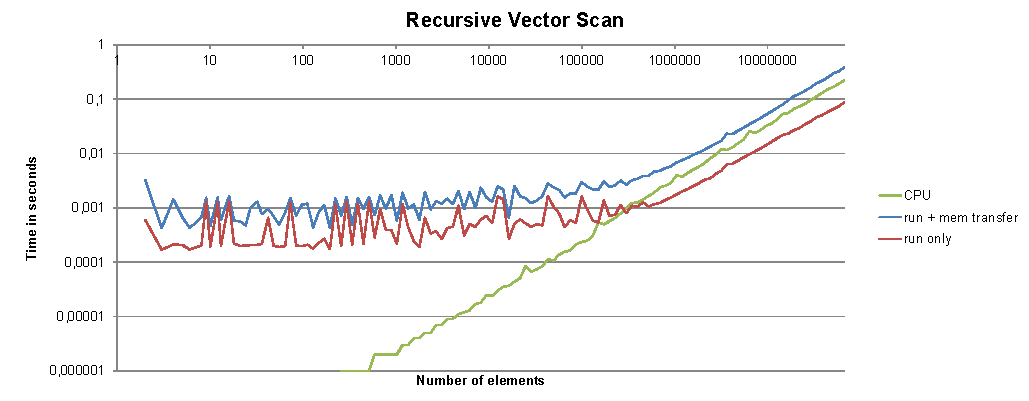
\includegraphics[width=1.0\linewidth]{scan_vector_chart}
\caption{A closer look to the benchmark of the recursive vector scan from section \ref{sec:scan_vector}. It points out how much time is wasted by memory transfers.
%The chart is based on the benchmark data in appendix section \ref{sec:scan_chart_data}.
Note that both axis are of logarithmic scale. }
\label{fig:scan_mem_transfer_chart}
\end{figure}

\pagebreak

\section{Further implementations}
Beside the presented kernels a further approach has been implemented and benchmarked which has not been covered. However some experiences may help future developers.

\begin{description}
	\item[Bank conflict avoidance] \hfill \\
	The GPU Gems 3 chapter about scan \cite{gpu_gems_3_chapter_39} also talks about avoiding bank conflicts occurring in the kernel in chapter \ref{sec:scan_work_efficient} where blocks are scanned in local memory. Both recursive scan implementations (chapters \ref{sec:scan_recursive} and \ref{sec:scan_vector}) have been implemented using the presented approach to avoid bank conflicts. However, the time required to calculate the conflict free offsets to local memory compensates for the time won by faster local memory access.
\end{description}

Furthermore, several libraries exist supporting GPGPU accelerated scans.

\begin{description}
   \item[clpp \cite{clpp}] \hfill \\
   The OpenCL Data Parallel Primitives Library is an open source and freely available library offering a few GPU primitives such as a scan and sort implementation. However, the project seems to be inactive (last release in July 2011).
   \item[ArrayFire \cite{arrayfire}] \hfill \\
   ArrayFire is a commercial GPU software acceleration library provided by AccelerEyes. It provides a lot of GPGPU accelerated algorithms using CUDA and OpenCL including scan.
%   \item[Apple \cite{apple_scan}] \hfill \\
%   Apple provides an example implementation of a parallel prefix sum using OpenCL in their Mac Developer Library.
%   \item[AMD \cite{amd_app_sdk}] \hfill \\
%   AMD also provides an example implementation of scan as part of their APP SDK.
%   \item[NVIDIA \cite{nvidia_opencl_samples}] \hfill \\
%   Finally, scan is also part of NVIDIA's OpenCL example codes which can be downloaded from their website.
\end{description}

\section{Summary and conclusion}
In this chapter we have seen how a sequential algorithm like the all-prefix-sum can be parallelized for GPUs. A tree based approach using several passes delivered good results. Also the idea of solving the problem in smaller sub groups which are than merged into the global result proofed to be successful. Both concepts are common patterns when trying to port sequential CPU code to a GPU. However, we did also learn that using a GPU does not always result in a performance boost, despite their enormous power. So does the final scan only perform three times faster than the CPU implementation excluding memory transfer. If the time for copying the data to and from the GPU's main memory is included, we would be better off staying with the CPU. This is a problem for many fast algorithms operating on larger chunks of memory. Nevertheless, a fast GPU implementation of such primitives can still be needed in cases where the input and output data is already present or consumed on the GPU. This is the case when input data is produced on the GPU (e.g., scanning image data from a rendering process) or present as input for other purposes (other algorithms, data for rendering). Also the output may be directly used by the GPU (e.g using scan as part of a filtering routine generating a list of objects to render). Even if a GPU algorithm would be slower in run time than a CPU version it might still outperform the CPU variant including memory transfer to and from the systems main memory.
